\problemset{Комбинаторика и теория графов}
\problemset{Индивидуальное домашнее задание №LO}	

\renewcommand*{\proofname}{Решение}

%%%%%%%%%%%%%% ЗАДАНИЕ №1 %%%%%%%%%%%%%%
%% Условие задания №1
\begin{problem}
    
    М=\{33, 97, 69, 71, 42, 49, 51, 59\}\newline
	Бинарное отношение задано выражением: \newline
  1) $$ F_{1}(x,y)=1\Leftrightarrow\exists z\in M:(x-z)(y-z)<0\newline$$
  2) $$ F_{1}(x,y)=1\Leftrightarrow x>=y\newline$$
  3) $$ F_{1}(x,y)=1\Leftrightarrow [x/2]=[y/2] \newline$$
  4) $$ F_{1}(x,y)=1\Leftrightarrow (x^2 - y^3) \vdots 2\newline$$
  5) $$ F_{1}(x,y)=1\Leftrightarrow |x - y| < 6\newline$$
 \newline
 Проверить, является ли бинарное отношение (далее -- б.о.) -- рефлексивным, арефлексивным, симметричным, антисимметричным, асимметричным, транзитивным.
\end{problem}

%% Решение задания №1
\begin{proof}
1)    Для удобства расположим числа, входящие в мн-во М, в порядке возрастания и построим матрицу для данного бинарного отношения:
	$$ \left( \begin{array}{c c c c c c c c c} 
   & 33 & 42 & 49 & 51 & 59 & 69 & 71 & 97 \\
 
33 & 0 & 0 & 1 & 1 & 1 & 1 & 1 & 1 \\ 

42 & 0 & 0 & 0 & 1 & 1 & 1 & 1 & 1 \\

49 & 1 & 0 & 0 & 0 & 1 & 1 & 1 & 1 \\
 
51 & 1 & 1 & 0 & 0 & 0 & 1 & 1 & 1 \\
 
59 & 1 & 1 & 1 & 0 & 0 & 0 & 1 & 1 \\
 
69 & 1 & 1 & 1 & 1 & 0 & 0 & 0 & 1 \\
 
71 & 1 & 1 & 1 & 1 & 1 & 0 & 0 & 0 \\
 
97 & 1 & 1 & 1 & 1 & 1 & 1 & 0 & 0 \end {array} \right) $$ \newline

    Б.о. арефлексивно, тк на главной диагонали матрицы все 0.
    \newline
    Б.о. симметрично, тк матрица симметрична относительно главной диагонали.
    \newline
    Б.о. нетранзитивно, тк при возведении матрицы в квадрат появляются новые связи.
    \newline

2)     Для удобства расположим числа, входящие в мн-во М в порядке возрастания и построим матрицу для данного бинарного отношения:
	$$ \left( \begin{array}{c c c c c c c c c} 
  & 33 & 42 & 49 & 51 & 59 & 69 & 71 & 97 \\
 
33 & 1 & 0 & 1 & 0 & 1 & 1 & 0 & 1 \\ 

42 & 0 & 1 & 1 & 0 & 1 & 1 & 0 & 1 \\

49 & 0 & 0 & 1 & 0 & 1 & 1 & 0 & 0 \\
 
51 & 0 & 0 & 0 & 1 & 0 & 1 & 1 & 1 \\
 
59 & 0 & 0 & 0 & 0 & 1 & 0 & 0 & 0 \\
 
69 & 0 & 0 & 0 & 0 & 0 & 1 & 0 & 0 \\
 
71 & 0 & 0 & 0 & 0 & 0 & 0 & 1 & 1 \\
 
97 & 0 & 0 & 0 & 0 & 0 & 0 & 0 & 1 \end {array} \right) $$ \newline

    Б.о. рефлексивно, тк на главной диагонали матрицы все 1.
    \newline
    Б.о. транзитивно, тк при возведении матрицы в квадрат не появляются новые связи.
     \newline
    Б.о. антисимметрично, тк выполняется условие $x \geq y \wedge y \geq x \Rightarrow x = y$.
      \newline

3)     Для удобства расположим числа, входящие в мн-во М в порядке возрастания и построим матрицу для данного бинарного отношения:
	$$ \left( \begin{array}{c c c c c c c c c} 
  & 33 & 42 & 49 & 51 & 59 & 69 & 71 & 97 \\
 
33 & 1 & 0 & 0 & 0 & 0 & 0 & 0 & 0 \\ 

42 & 0 & 1 & 0 & 0 & 0 & 0 & 0 & 0 \\

49 & 0 & 0 & 1 & 0 & 0 & 0 & 0 & 0 \\
 
51 & 0 & 0 & 0 & 1 & 0 & 0 & 0 & 0 \\
 
59 & 0 & 0 & 0 & 0 & 1 & 0 & 0 & 0 \\
 
69 & 0 & 0 & 0 & 0 & 0 & 1 & 0 & 0 \\
 
71 & 0 & 0 & 0 & 0 & 0 & 0 & 1 & 0 \\
 
97 & 0 & 0 & 0 & 0 & 0 & 0 & 0 & 1 \end {array} \right) $$
 Б.о. рефлексивно, тк на главной диагонали матрицы все 1.
    \newline
     Б.о. симметрично, тк матрица симметрична относительно главной диагонали.
    \newline
     Б.о. антисимметрично, тк выполняется условие $x \geq y \wedge y \geq x \Rightarrow x = y$.
    \newline
    Б.о. транзитивно, тк при возведении матрицы в квадрат не появляются новые связи.\newline

4) Для удобства расположим числа, входящие в мн-во М в порядке возрастания и построим матрицу для данного бинарного отношения:
	$$ \left( \begin{array}{c c c c c c c c c} 
  & 33 & 42 & 49 & 51 & 59 & 69 & 71 & 97 \\
 
33 & 1 & 0 & 1 & 1 & 1 & 1 & 1 & 1 \\ 

42 & 0 & 1 & 0 & 0 & 0 & 0 & 0 & 0 \\

49 & 1 & 0 & 1 & 1 & 1 & 1 & 1 & 1 \\ 
 
51 & 1 & 0 & 1 & 1 & 1 & 1 & 1 & 1 \\ 
 
59 & 1 & 0 & 1 & 1 & 1 & 1 & 1 & 1 \\ 
 
69 & 1 & 0 & 1 & 1 & 1 & 1 & 1 & 1 \\ 
 
71 & 1 & 0 & 1 & 1 & 1 & 1 & 1 & 1 \\ 
 
97 & 1 & 0 & 1 & 1 & 1 & 1 & 1 & 1  \end {array} \right) $$
 Б.о. рефлексивно, тк на главной диагонали матрицы все 1.
    \newline
     Б.о. симметрично, тк матрица симметрична относительно главной диагонали.
    \newline
    Б.о. транзитивно, тк при возведении матрицы в квадрат не появляются новые связи.
     \newline

5)     Для удобства расположим числа, входящие в мн-во М в порядке возрастания и построим матрицу для данного бинарного отношения:
	$$ \left( \begin{array}{c c c c c c c c c} 
  & 33 & 42 & 49 & 51 & 59 & 69 & 71 & 97 \\
 
33 & 1 & 0 & 0 & 0 & 0 & 0 & 0 & 0 \\ 

42 & 0 & 1 & 0 & 0 & 0 & 0 & 0 & 0 \\

49 & 0 & 0 & 1 & 0 & 0 & 0 & 0 & 0 \\
 
51 & 0 & 0 & 0 & 1 & 1 & 0 & 0 & 0 \\
 
59 & 0 & 0 & 0 & 1 & 1 & 0 & 0 & 0 \\
 
69 & 0 & 0 & 0 & 0 & 0 & 1 & 1 & 0 \\
 
71 & 0 & 0 & 0 & 0 & 0 & 1 & 1 & 0 \\
 
97 & 0 & 0 & 0 & 0 & 0 & 0 & 0 & 1  \end {array} \right) $$

 Б.о. рефлексивно, тк на главной диагонали матрицы все 1.
    \newline
     Б.о. симметрично, тк матрица симметрична относительно главной диагонали.
    \newline
    Б.о. транзитивно, тк при возведении матрицы в квадрат не появляются новые связи.

\end{proof}

%%%%%%%%%%%%%% ЗАДАНИЕ №2 %%%%%%%%%%%%%%
%% Условие задания №2
\begin{problem}
	Постройте матрицу и граф этого б.о.
\end{problem}

%% Решение задания №2
\begin{proof}
Перед построением матрицы отсортируем вершины по возрастанию. Таким образом строчке(столбцу) с меньшим порядковым номером соответсвует вершина с меньшим значением, а строчке(столбцу) с большим порядковым номером -- вершина с большим значением. \newline
1) 	$$ \left( \begin{array}{c c c c c c c c c} 
   & 33 & 42 & 49 & 51 & 59 & 69 & 71 & 97 \\
 
33 & 0 & 0 & 1 & 1 & 1 & 1 & 1 & 1 \\ 

42 & 0 & 0 & 0 & 1 & 1 & 1 & 1 & 1 \\

49 & 1 & 0 & 0 & 0 & 1 & 1 & 1 & 1 \\
 
51 & 1 & 1 & 0 & 0 & 0 & 1 & 1 & 1 \\
 
59 & 1 & 1 & 1 & 0 & 0 & 0 & 1 & 1 \\
 
69 & 1 & 1 & 1 & 1 & 0 & 0 & 0 & 1 \\
 
71 & 1 & 1 & 1 & 1 & 1 & 0 & 0 & 0 \\
 
97 & 1 & 1 & 1 & 1 & 1 & 1 & 0 & 0 \end {array} \right) $$ \newline
 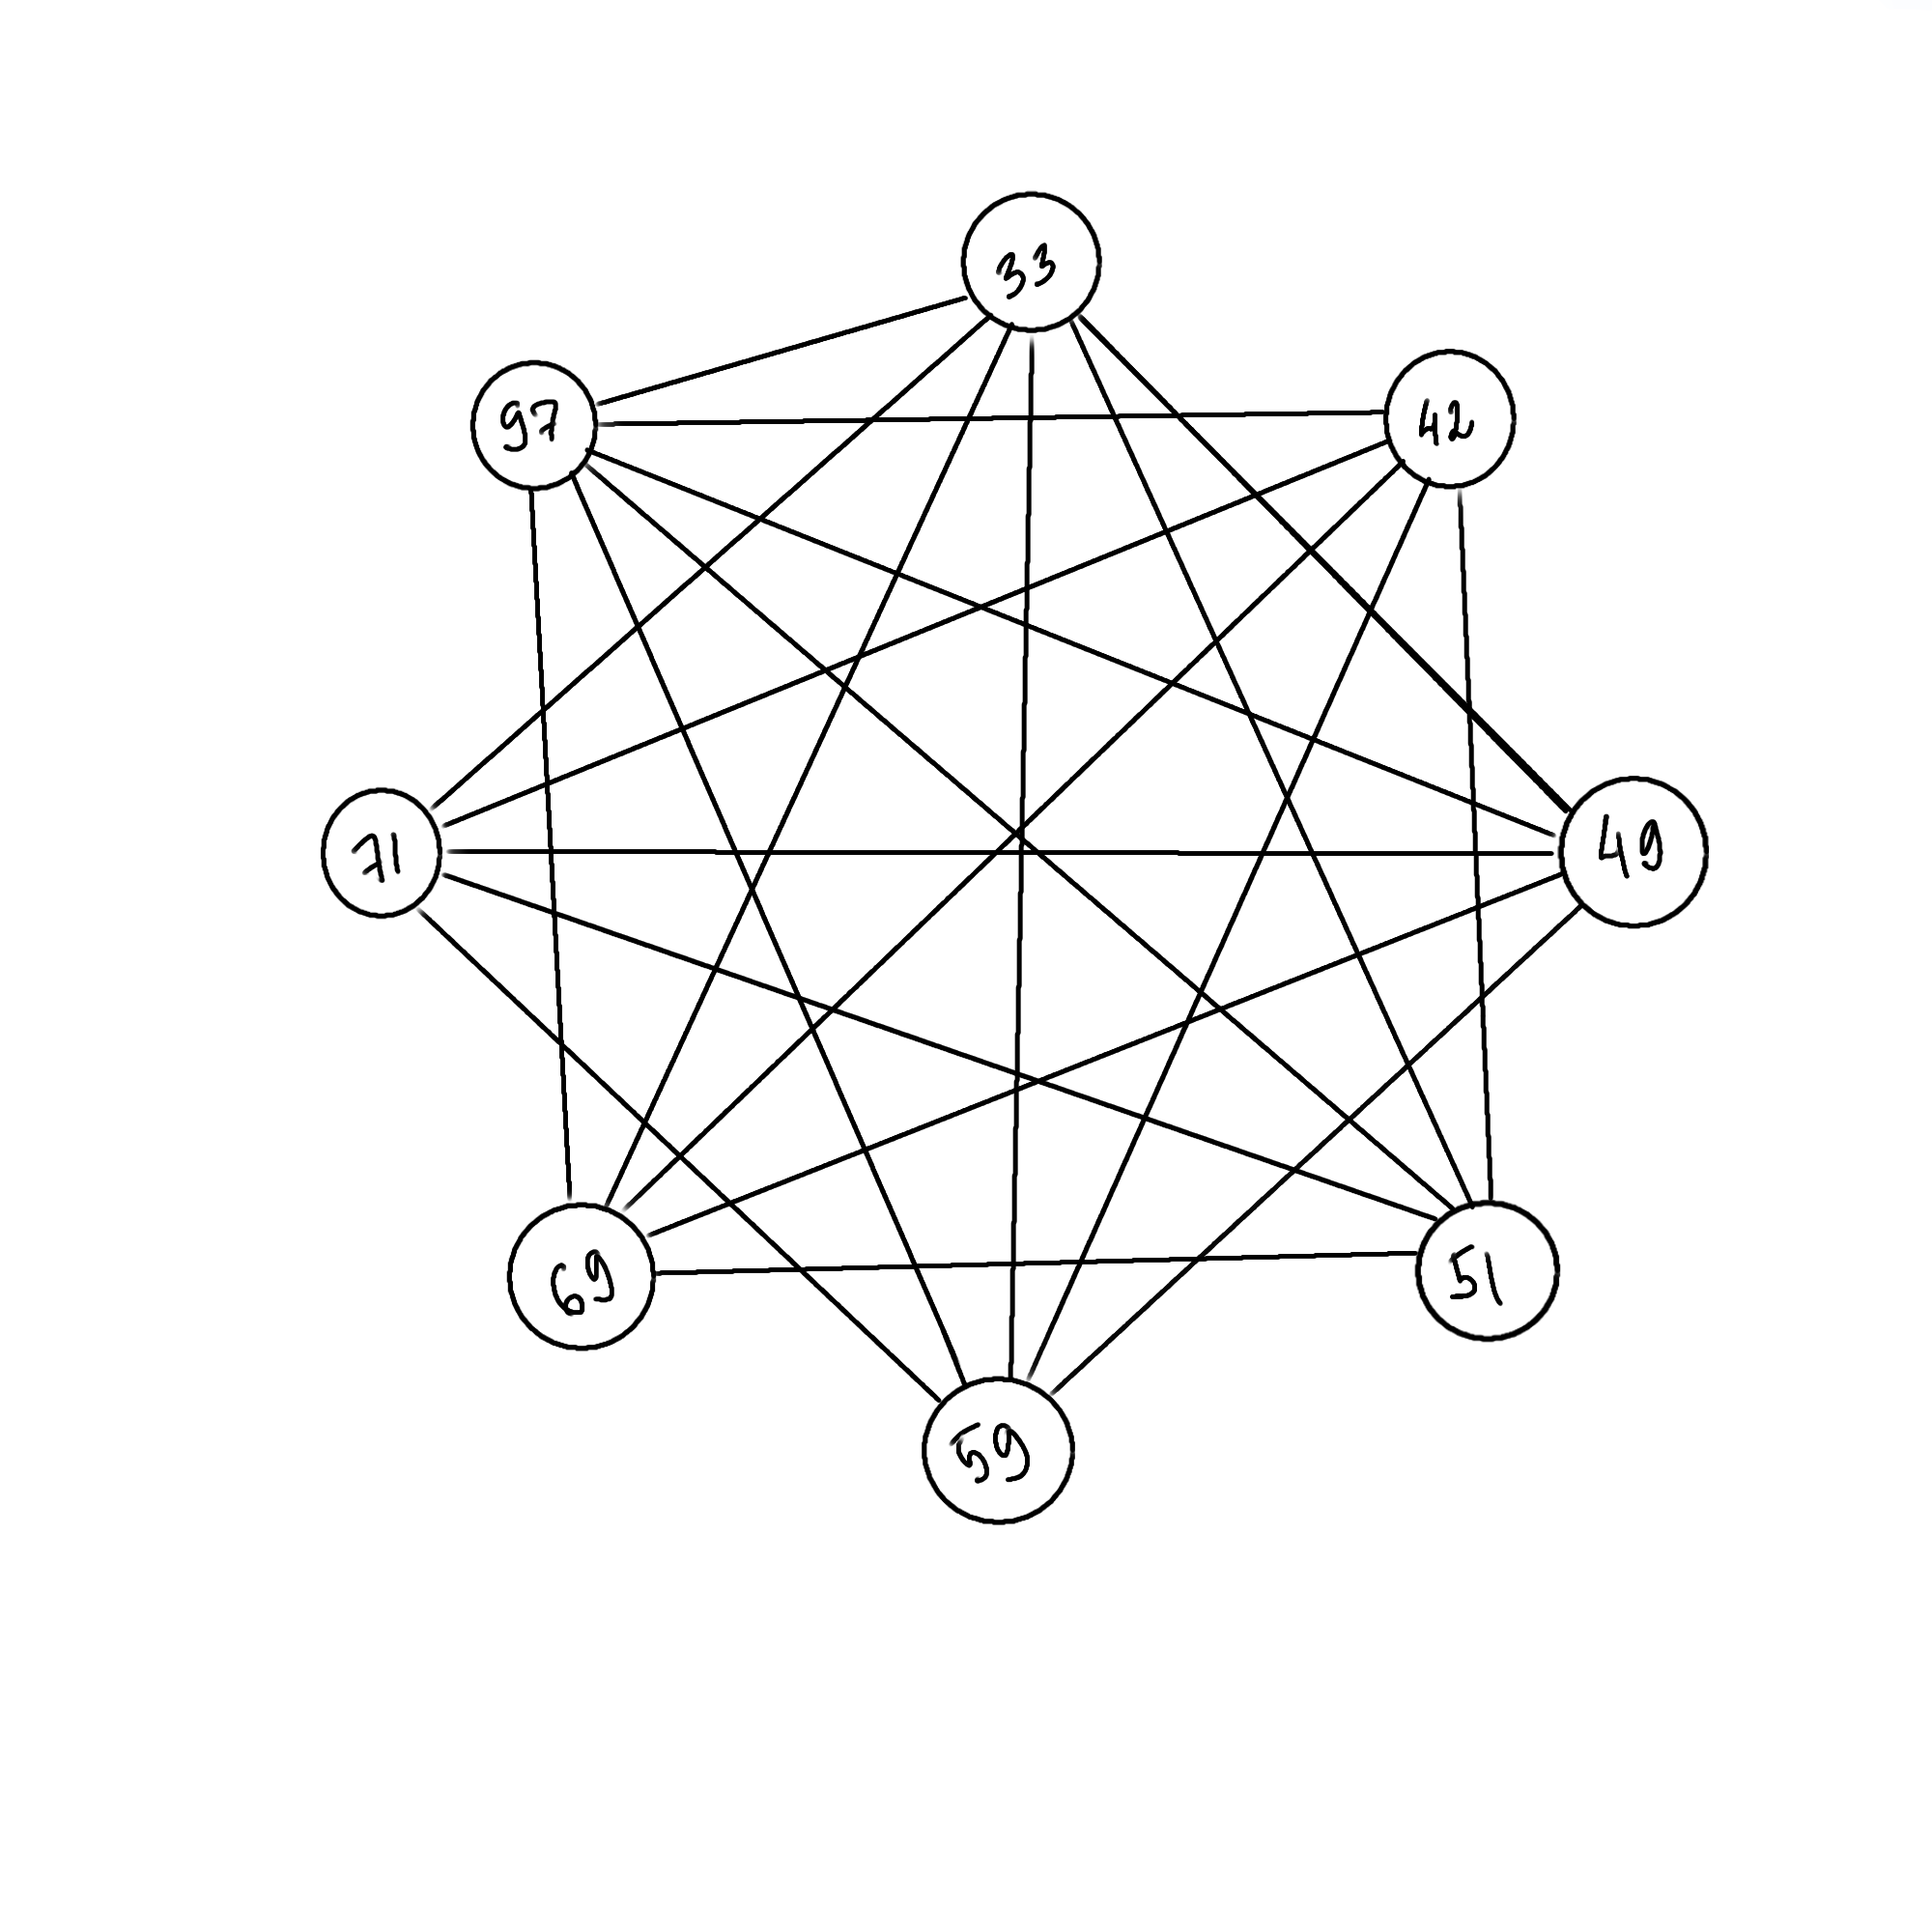
\includegraphics{граф1.png}
 
2)$$ \left( \begin{array}{c c c c c c c c c} 
  & 33 & 42 & 49 & 51 & 59 & 69 & 71 & 97 \\
 
33 & 1 & 0 & 1 & 0 & 1 & 1 & 0 & 1 \\ 

42 & 0 & 1 & 1 & 0 & 1 & 1 & 0 & 1 \\

49 & 0 & 0 & 1 & 0 & 1 & 1 & 0 & 0 \\
 
51 & 0 & 0 & 0 & 1 & 0 & 1 & 1 & 1 \\
 
59 & 0 & 0 & 0 & 0 & 1 & 0 & 0 & 0 \\
 
69 & 0 & 0 & 0 & 0 & 0 & 1 & 0 & 0 \\
 
71 & 0 & 0 & 0 & 0 & 0 & 0 & 1 & 1 \\
 
97 & 0 & 0 & 0 & 0 & 0 & 0 & 0 & 1 \end {array} \right) $$ \newline
 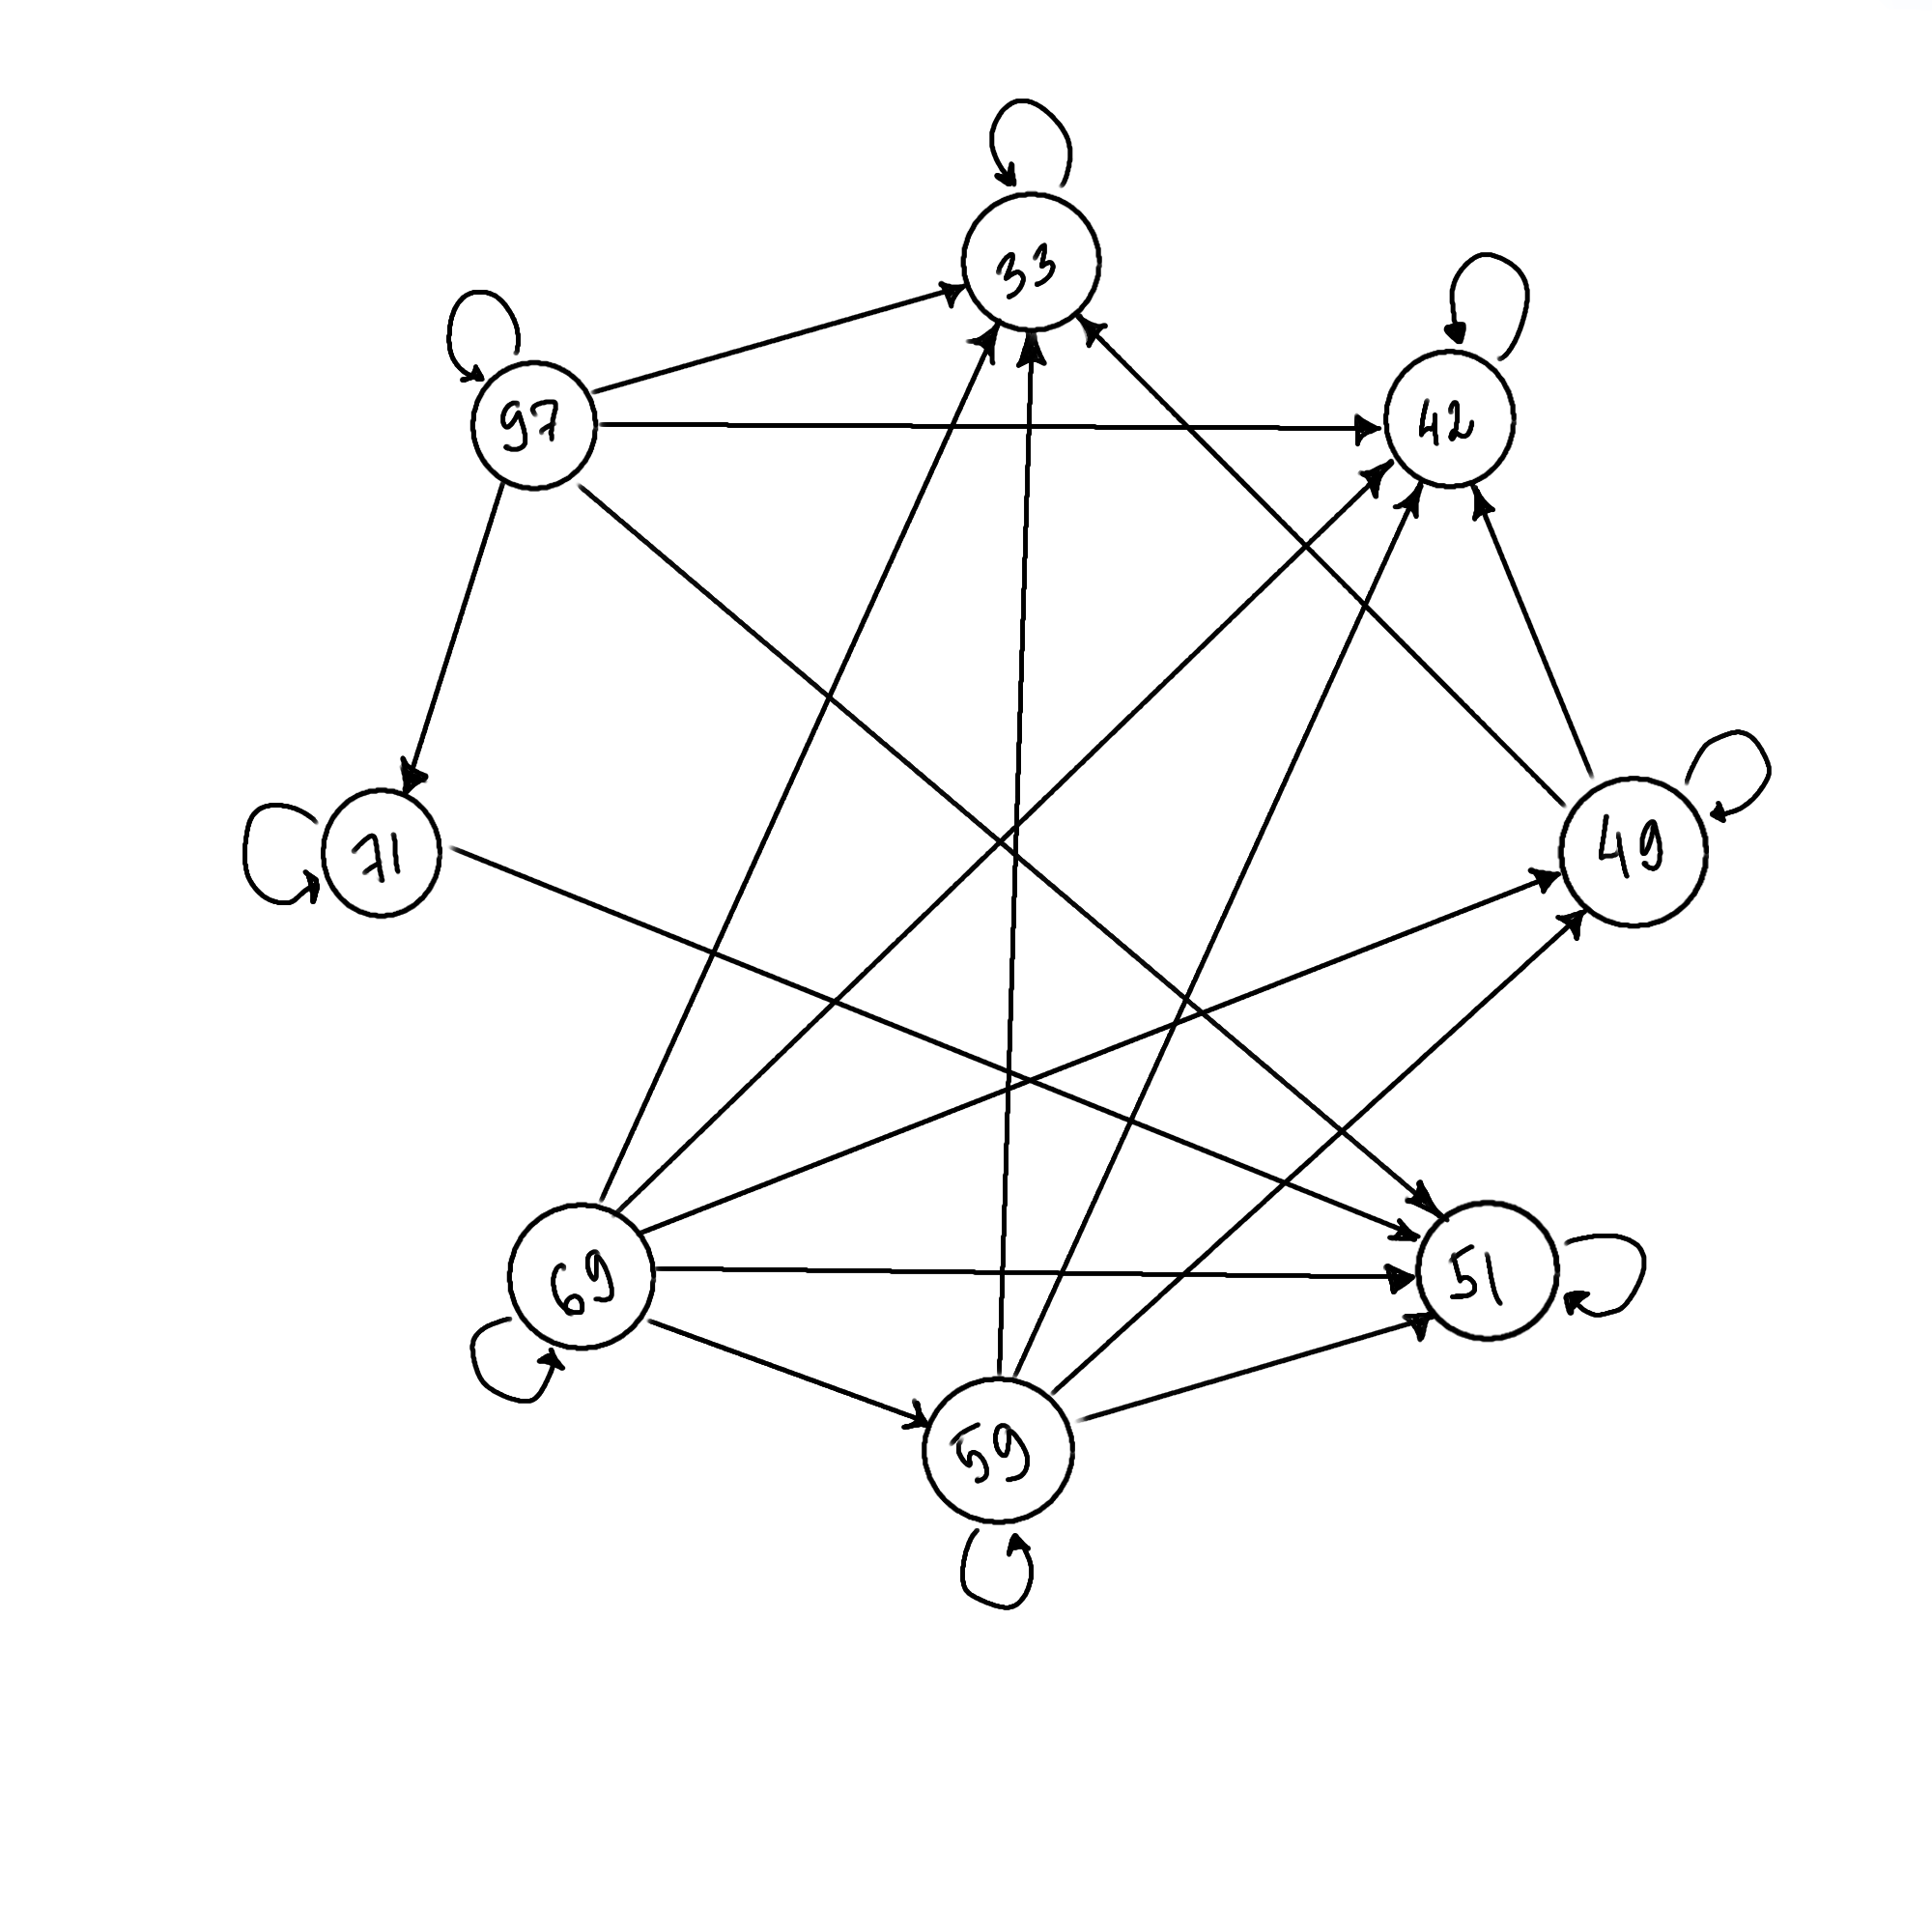
\includegraphics{граф2.png}

3)$$ \left( \begin{array}{c c c c c c c c c} 
  & 33 & 42 & 49 & 51 & 59 & 69 & 71 & 97 \\
 
33 & 1 & 0 & 0 & 0 & 0 & 0 & 0 & 0 \\ 

42 & 0 & 1 & 0 & 0 & 0 & 0 & 0 & 0 \\

49 & 0 & 0 & 1 & 0 & 0 & 0 & 0 & 0 \\
 
51 & 0 & 0 & 0 & 1 & 0 & 0 & 0 & 0 \\
 
59 & 0 & 0 & 0 & 0 & 1 & 0 & 0 & 0 \\
 
69 & 0 & 0 & 0 & 0 & 0 & 1 & 0 & 0 \\
 
71 & 0 & 0 & 0 & 0 & 0 & 0 & 1 & 0 \\
 
97 & 0 & 0 & 0 & 0 & 0 & 0 & 0 & 1 \end {array} \right) $$ \newline
 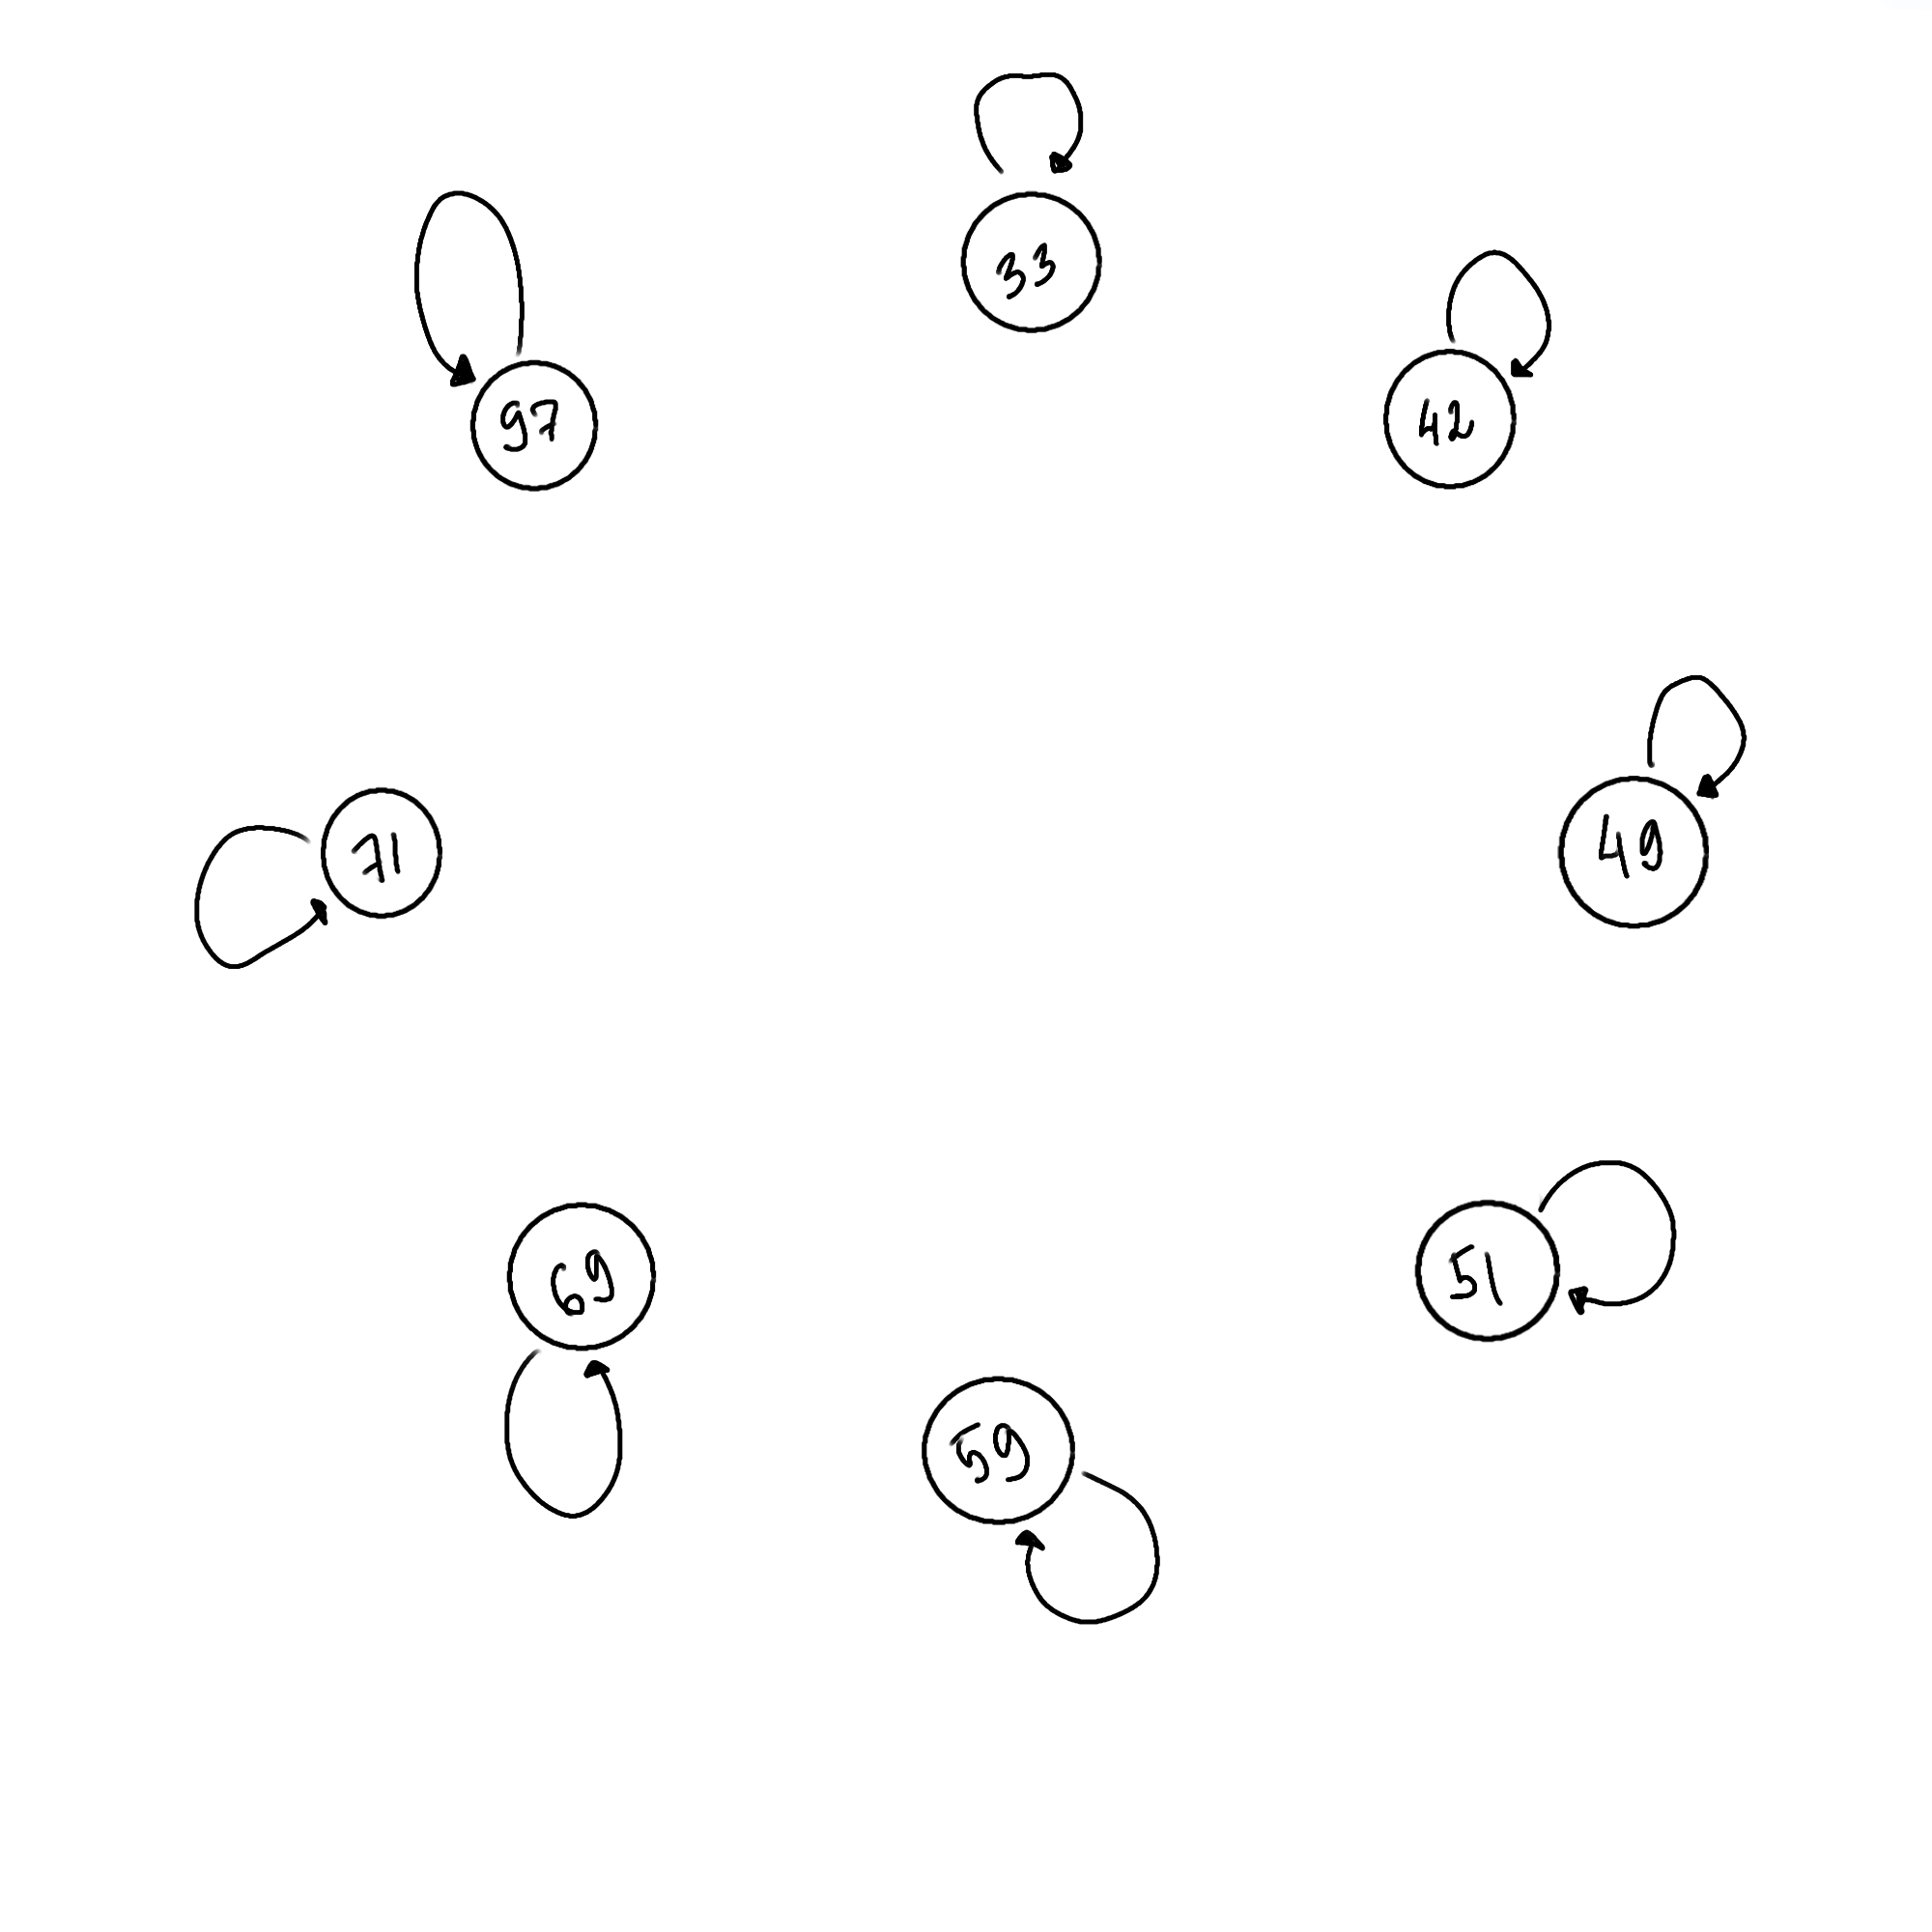
\includegraphics{граф3.png}

4)$$ \left( \begin{array}{c c c c c c c c c} 
  & 33 & 42 & 49 & 51 & 59 & 69 & 71 & 97 \\
 
33 & 1 & 0 & 1 & 1 & 1 & 1 & 1 & 1 \\ 

42 & 0 & 1 & 0 & 0 & 0 & 0 & 0 & 0 \\

49 & 1 & 0 & 1 & 1 & 1 & 1 & 1 & 1 \\ 
 
51 & 1 & 0 & 1 & 1 & 1 & 1 & 1 & 1 \\ 
 
59 & 1 & 0 & 1 & 1 & 1 & 1 & 1 & 1 \\ 
 
69 & 1 & 0 & 1 & 1 & 1 & 1 & 1 & 1 \\ 
 
71 & 1 & 0 & 1 & 1 & 1 & 1 & 1 & 1 \\ 
 
97 & 1 & 0 & 1 & 1 & 1 & 1 & 1 & 1  \end {array} \right) $$ \newline
 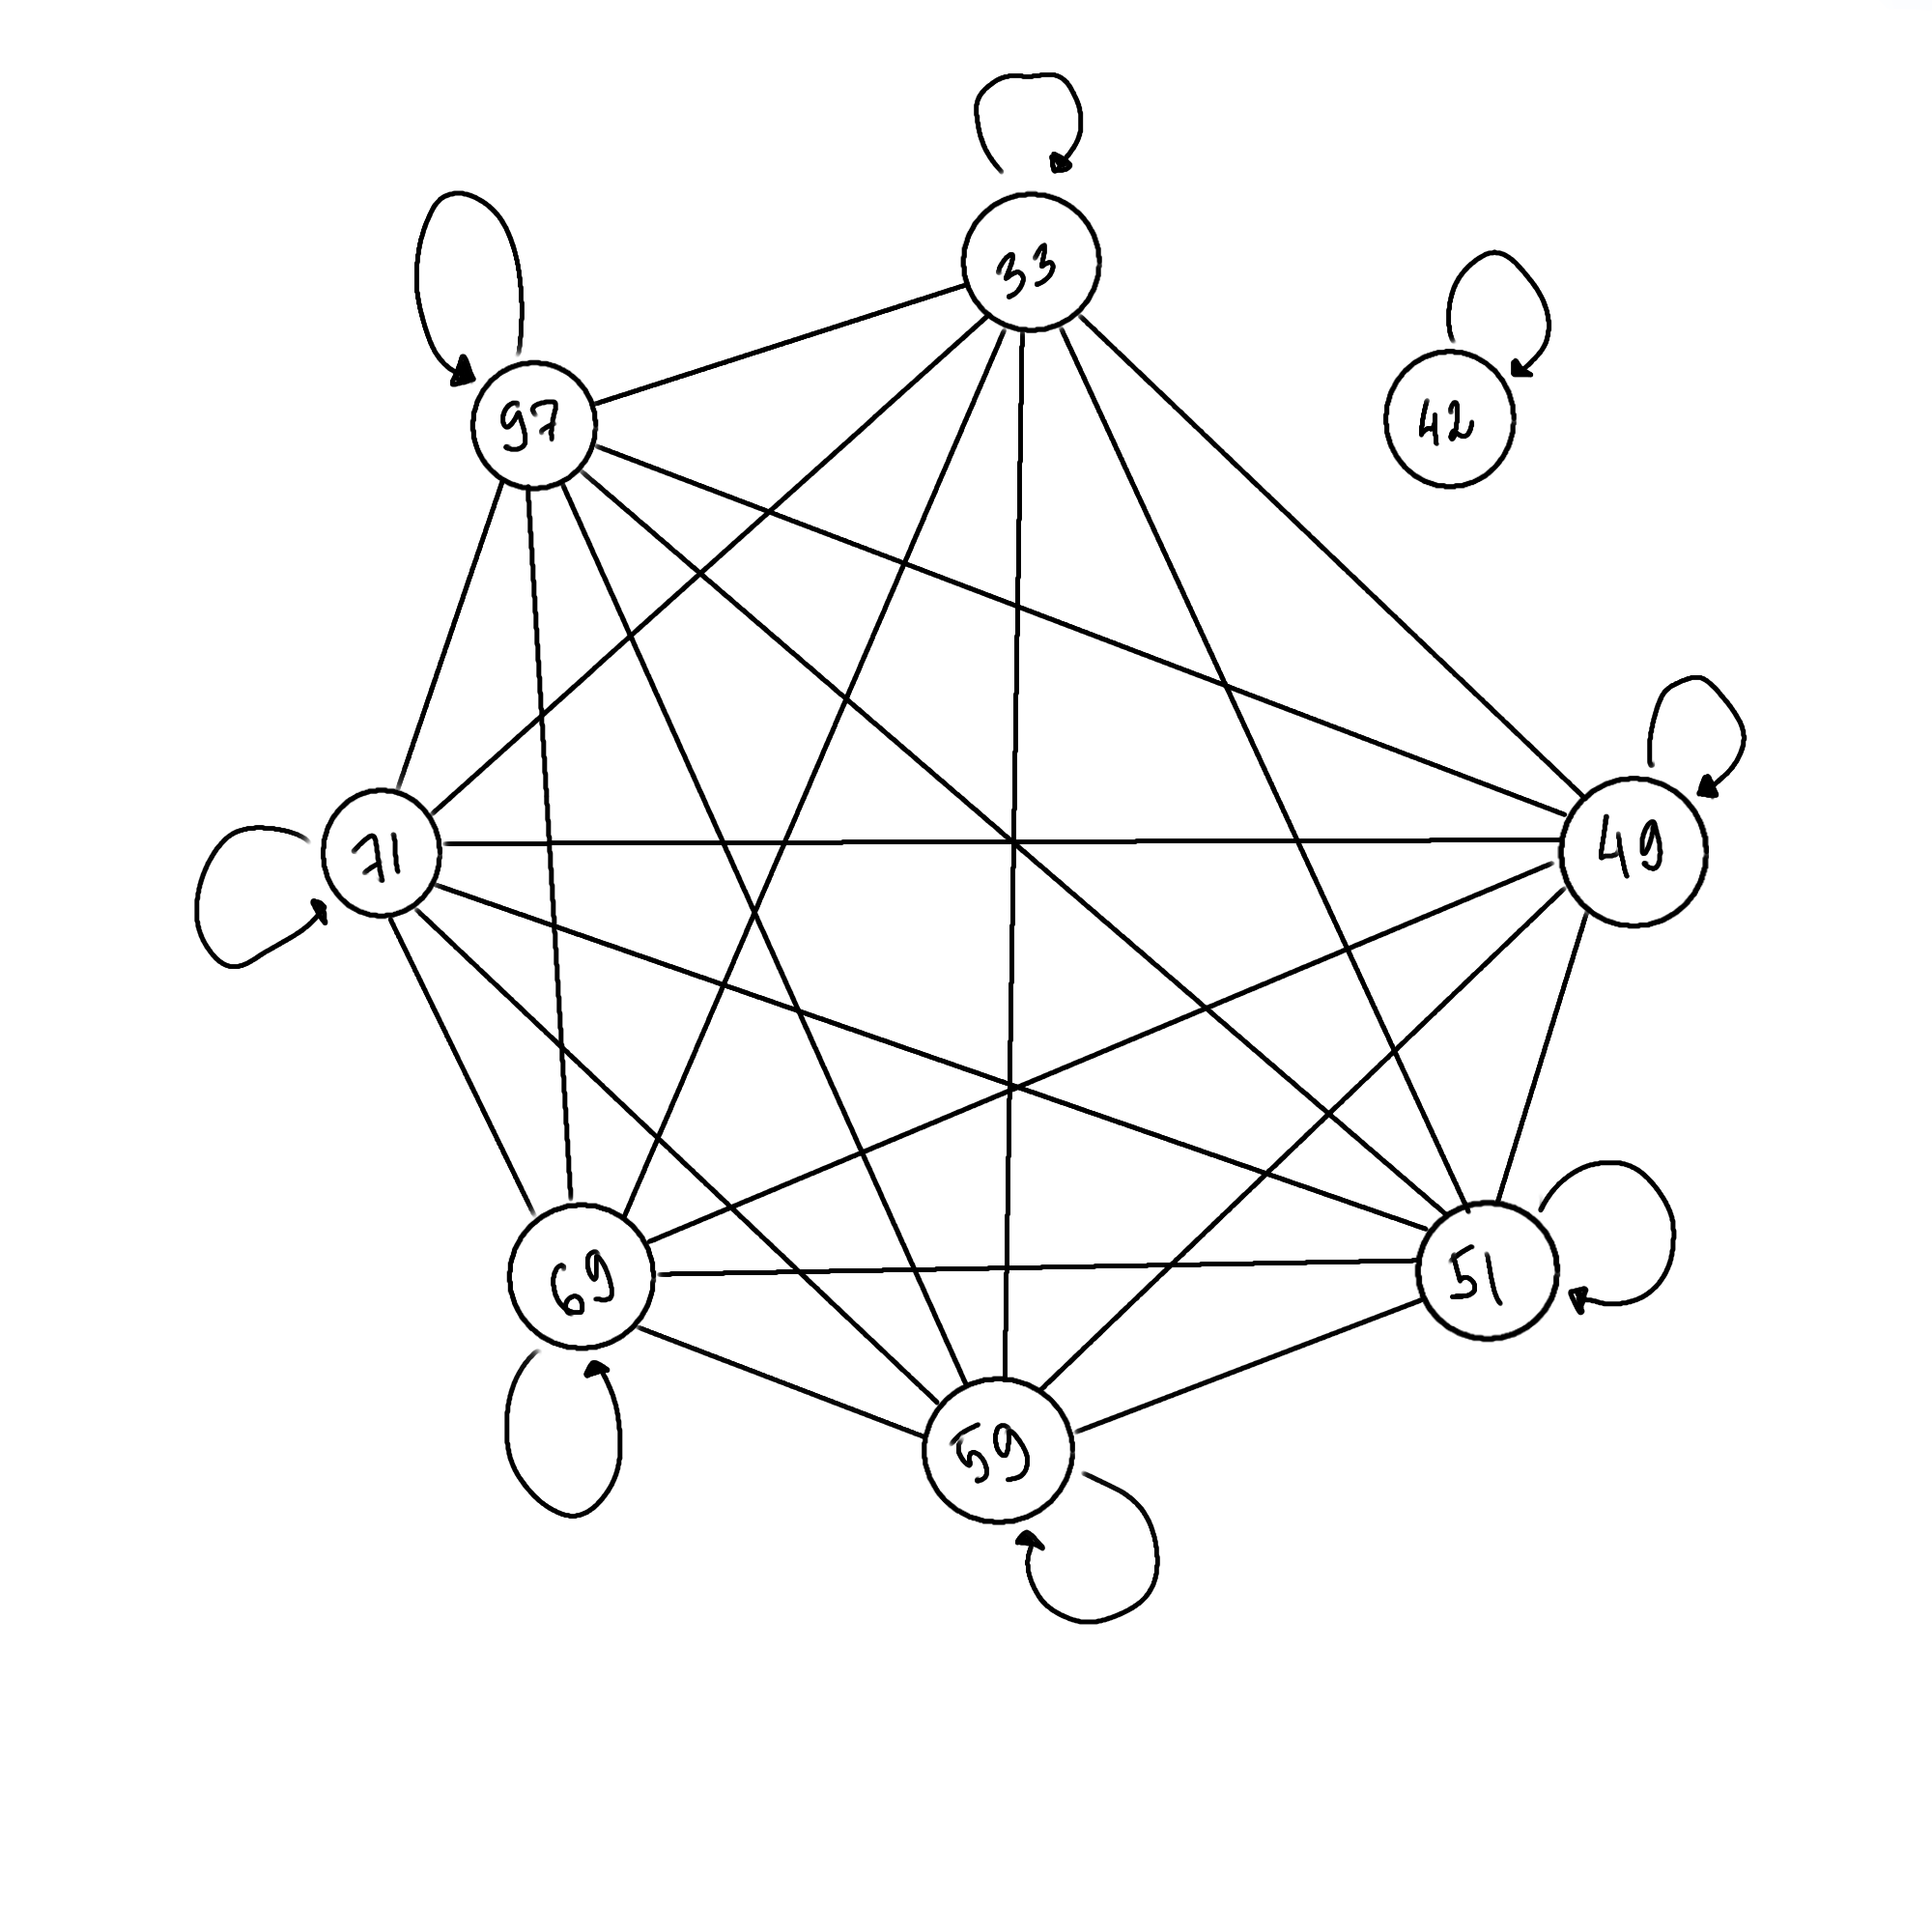
\includegraphics{граф4.png}

5)	$$ \left( \begin{array}{c c c c c c c c c} 
  & 33 & 42 & 49 & 51 & 59 & 69 & 71 & 97 \\
 
33 & 1 & 0 & 0 & 0 & 0 & 0 & 0 & 0 \\ 

42 & 0 & 1 & 0 & 0 & 0 & 0 & 0 & 0 \\

49 & 0 & 0 & 1 & 0 & 0 & 0 & 0 & 0 \\
 
51 & 0 & 0 & 0 & 1 & 1 & 0 & 0 & 0 \\
 
59 & 0 & 0 & 0 & 1 & 1 & 0 & 0 & 0 \\
 
69 & 0 & 0 & 0 & 0 & 0 & 1 & 1 & 0 \\
 
71 & 0 & 0 & 0 & 0 & 0 & 1 & 1 & 0 \\
 
97 & 0 & 0 & 0 & 0 & 0 & 0 & 0 & 1  \end {array} \right) $$\newline
 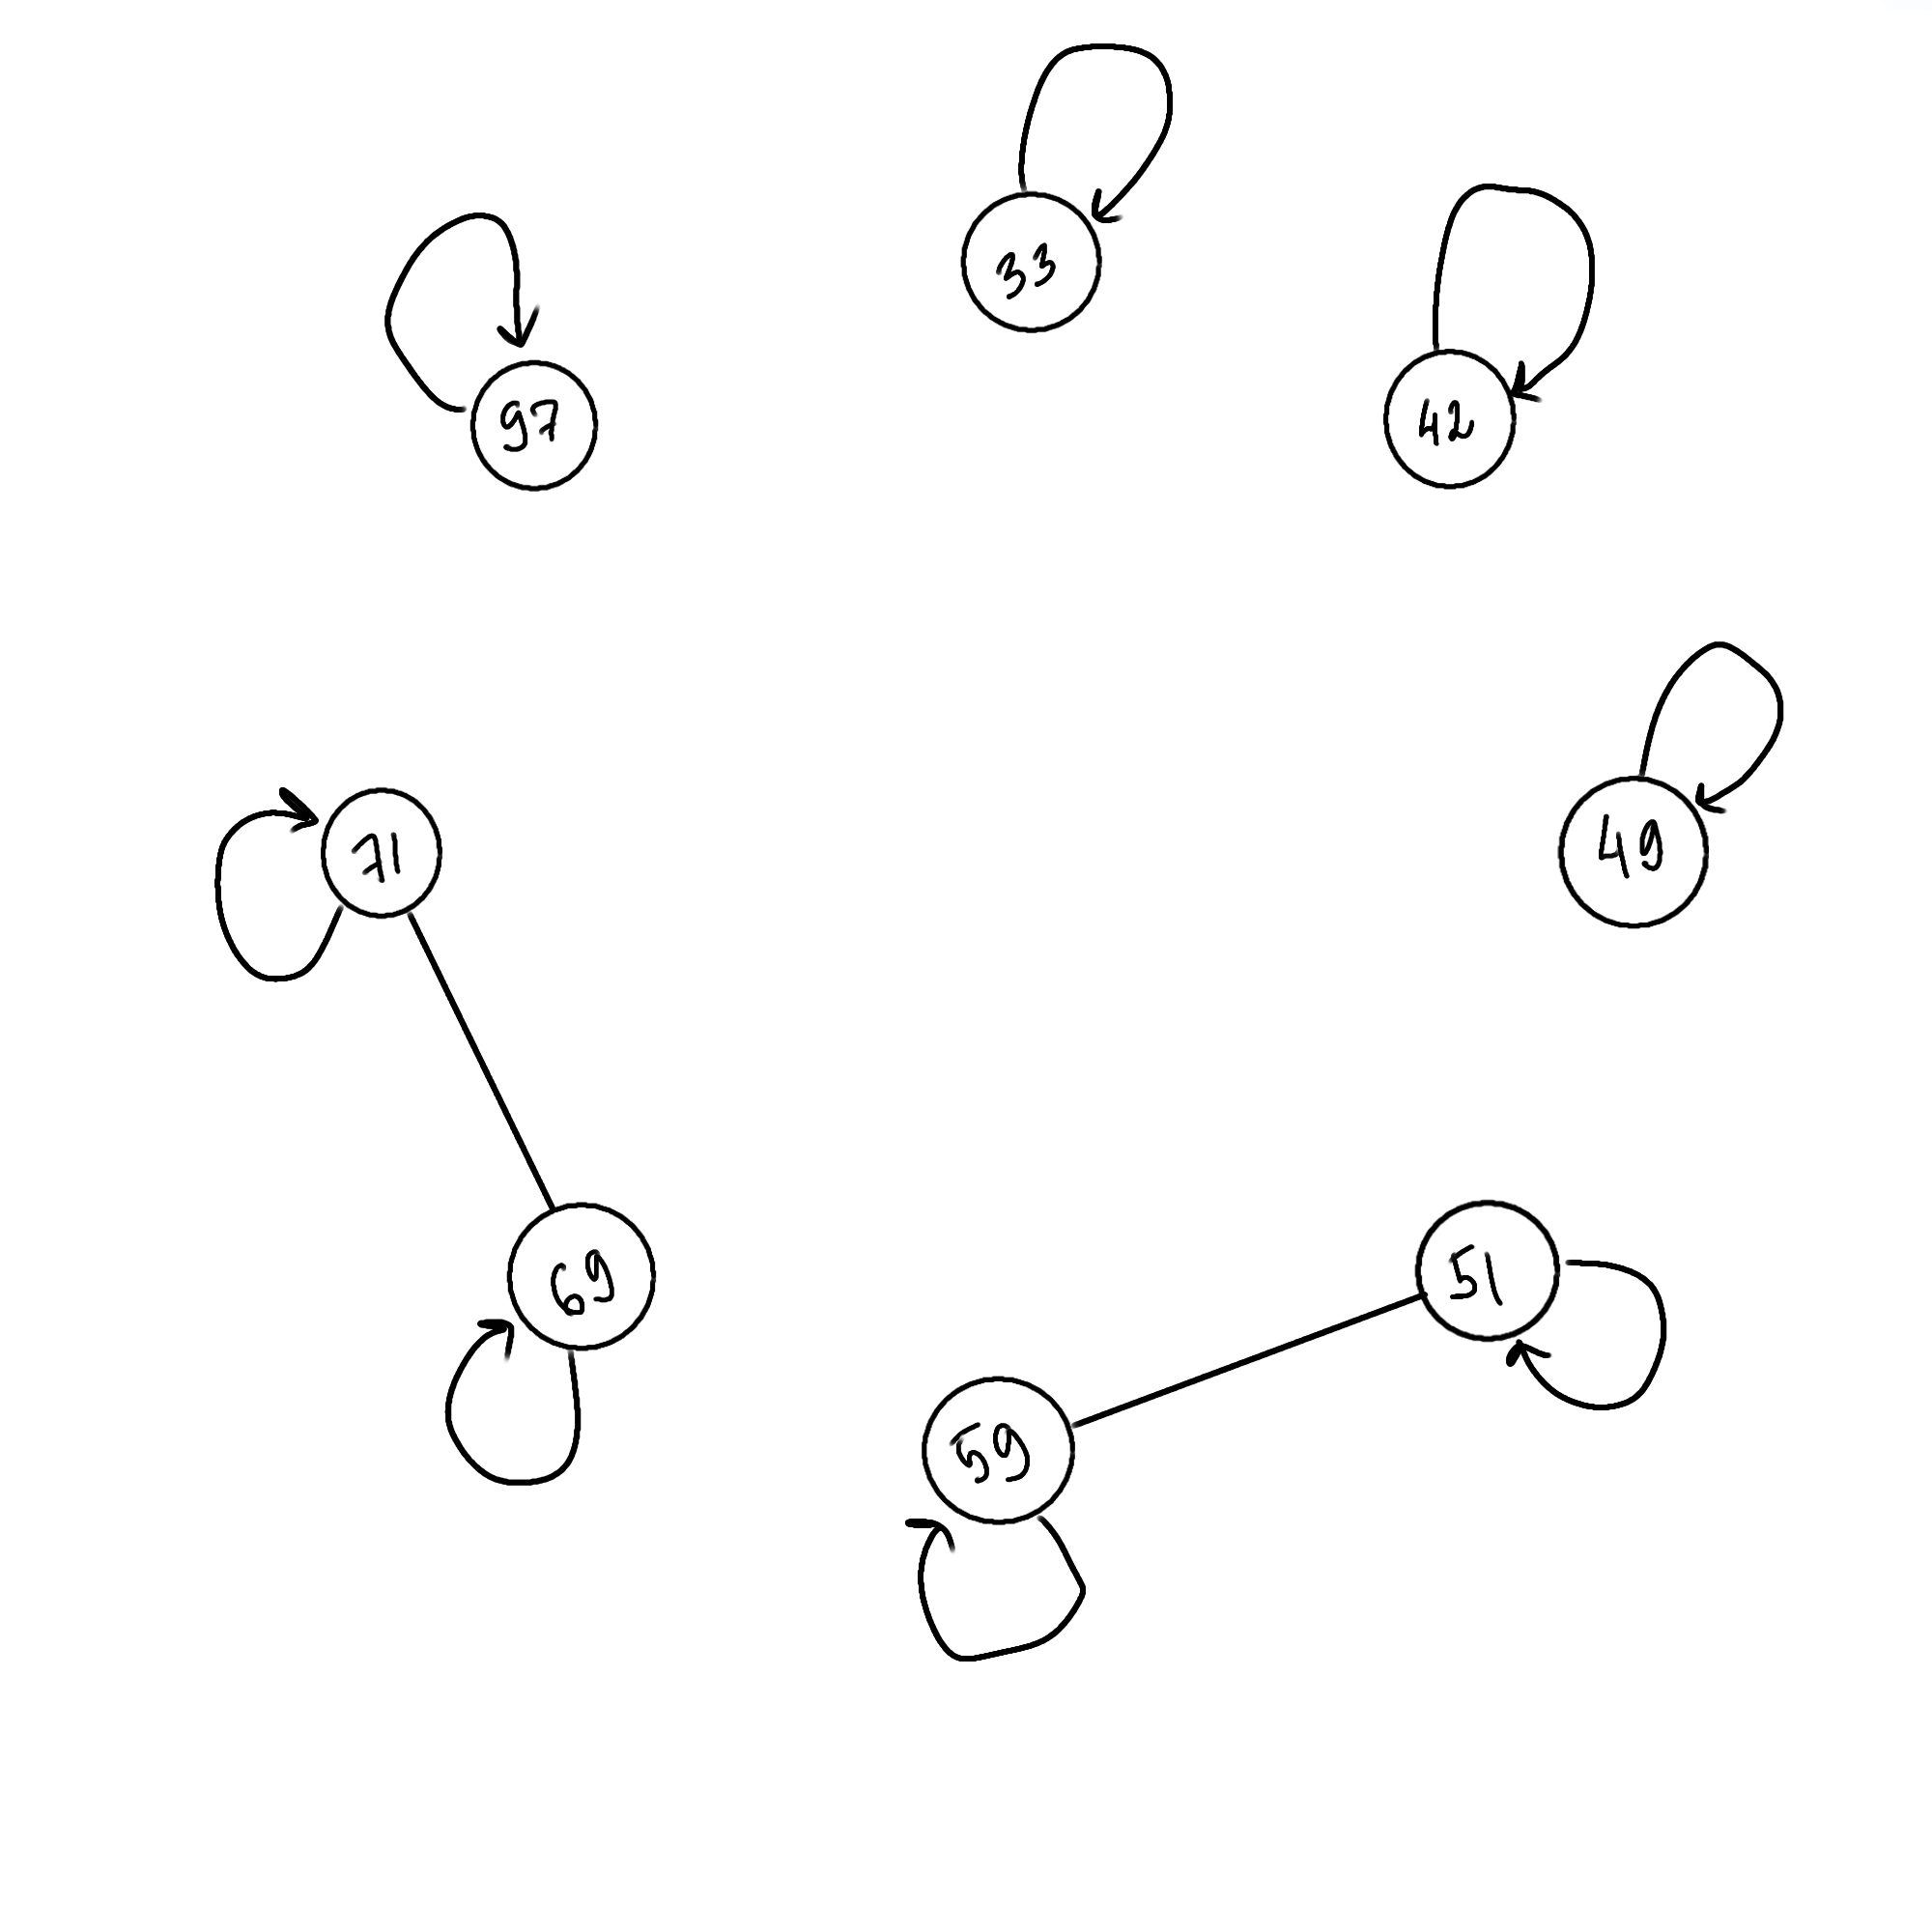
\includegraphics{граф5.png}
\end{proof}

%%%%%%%%%%%%%% ЗАДАНИЕ №3 %%%%%%%%%%%%%%
%% Условие задания №3
\begin{problem}
	Определить, является ли это б.о. отношением эквивалентности, частичного порядка, линейного порядка, строгого порядка.
\end{problem}

%% Решение задания №3
\begin{proof}
	1) Данное б.о. не является никаким из перечисленных, тк арефлексивно, симметрично и нетранзитивно.\newline
    2) Б. о. является отношением частичного порядка, тк рефлексивно, антисимметрично и транзитивно.\newline
    3) Б. о. является отношением эквиваллентности и частичного порядка, тк рефлексивно, симметрично, антисимметрично и трназитивно.\newline
    4) Б. о. является отношением эквиваллентности, тк рефлексивно, симметрично и транзитивно.\newline
    5) Б. о. является отношением эквиваллентности, тк рефлексивно, симметрично и транзитивно.\newline
\end{proof}
%%%%%%%%%%%%%% ЗАДАНИЕ №4 %%%%%%%%%%%%%%
%% Условие задания №4
\begin{problem}
	Для отношений эквивалентности построить классы эквивалентности.
\end{problem}

%% Решение задания №4
\begin{proof}
   1) данное б.о. не является отношением эквивалентности\newline
   2) данное б.о. не является отношением эквивалентности\newline
   3) \{ 33\}\{ 42\}\{ 49\}\{ 51\}\{ 59\}\{ 69\}\{ 71\}\{ 97\}\newline
   4) \{ 33, 49, 51, 59, 69, 71, 97\}\{ 42\}\newline
   5) \{ 33\}\{ 42\}\{ 49\}\{ 51, 59\}\{ 69\}\{ 71, 97\}\newline
\end{proof}
%%%%%%%%%%%%%% ЗАДАНИЕ №5 %%%%%%%%%%%%%%
%% Условие задания №5
\begin{problem}
	Для отношений частичного порядка применить алгоритм топологической сортировки и получить отношение линейного порядка.
\end{problem}

%% Решение задания №5
\begin{proof}
    1) данное б.о. не является отношением частичного порядка\newline
    2)\newline
    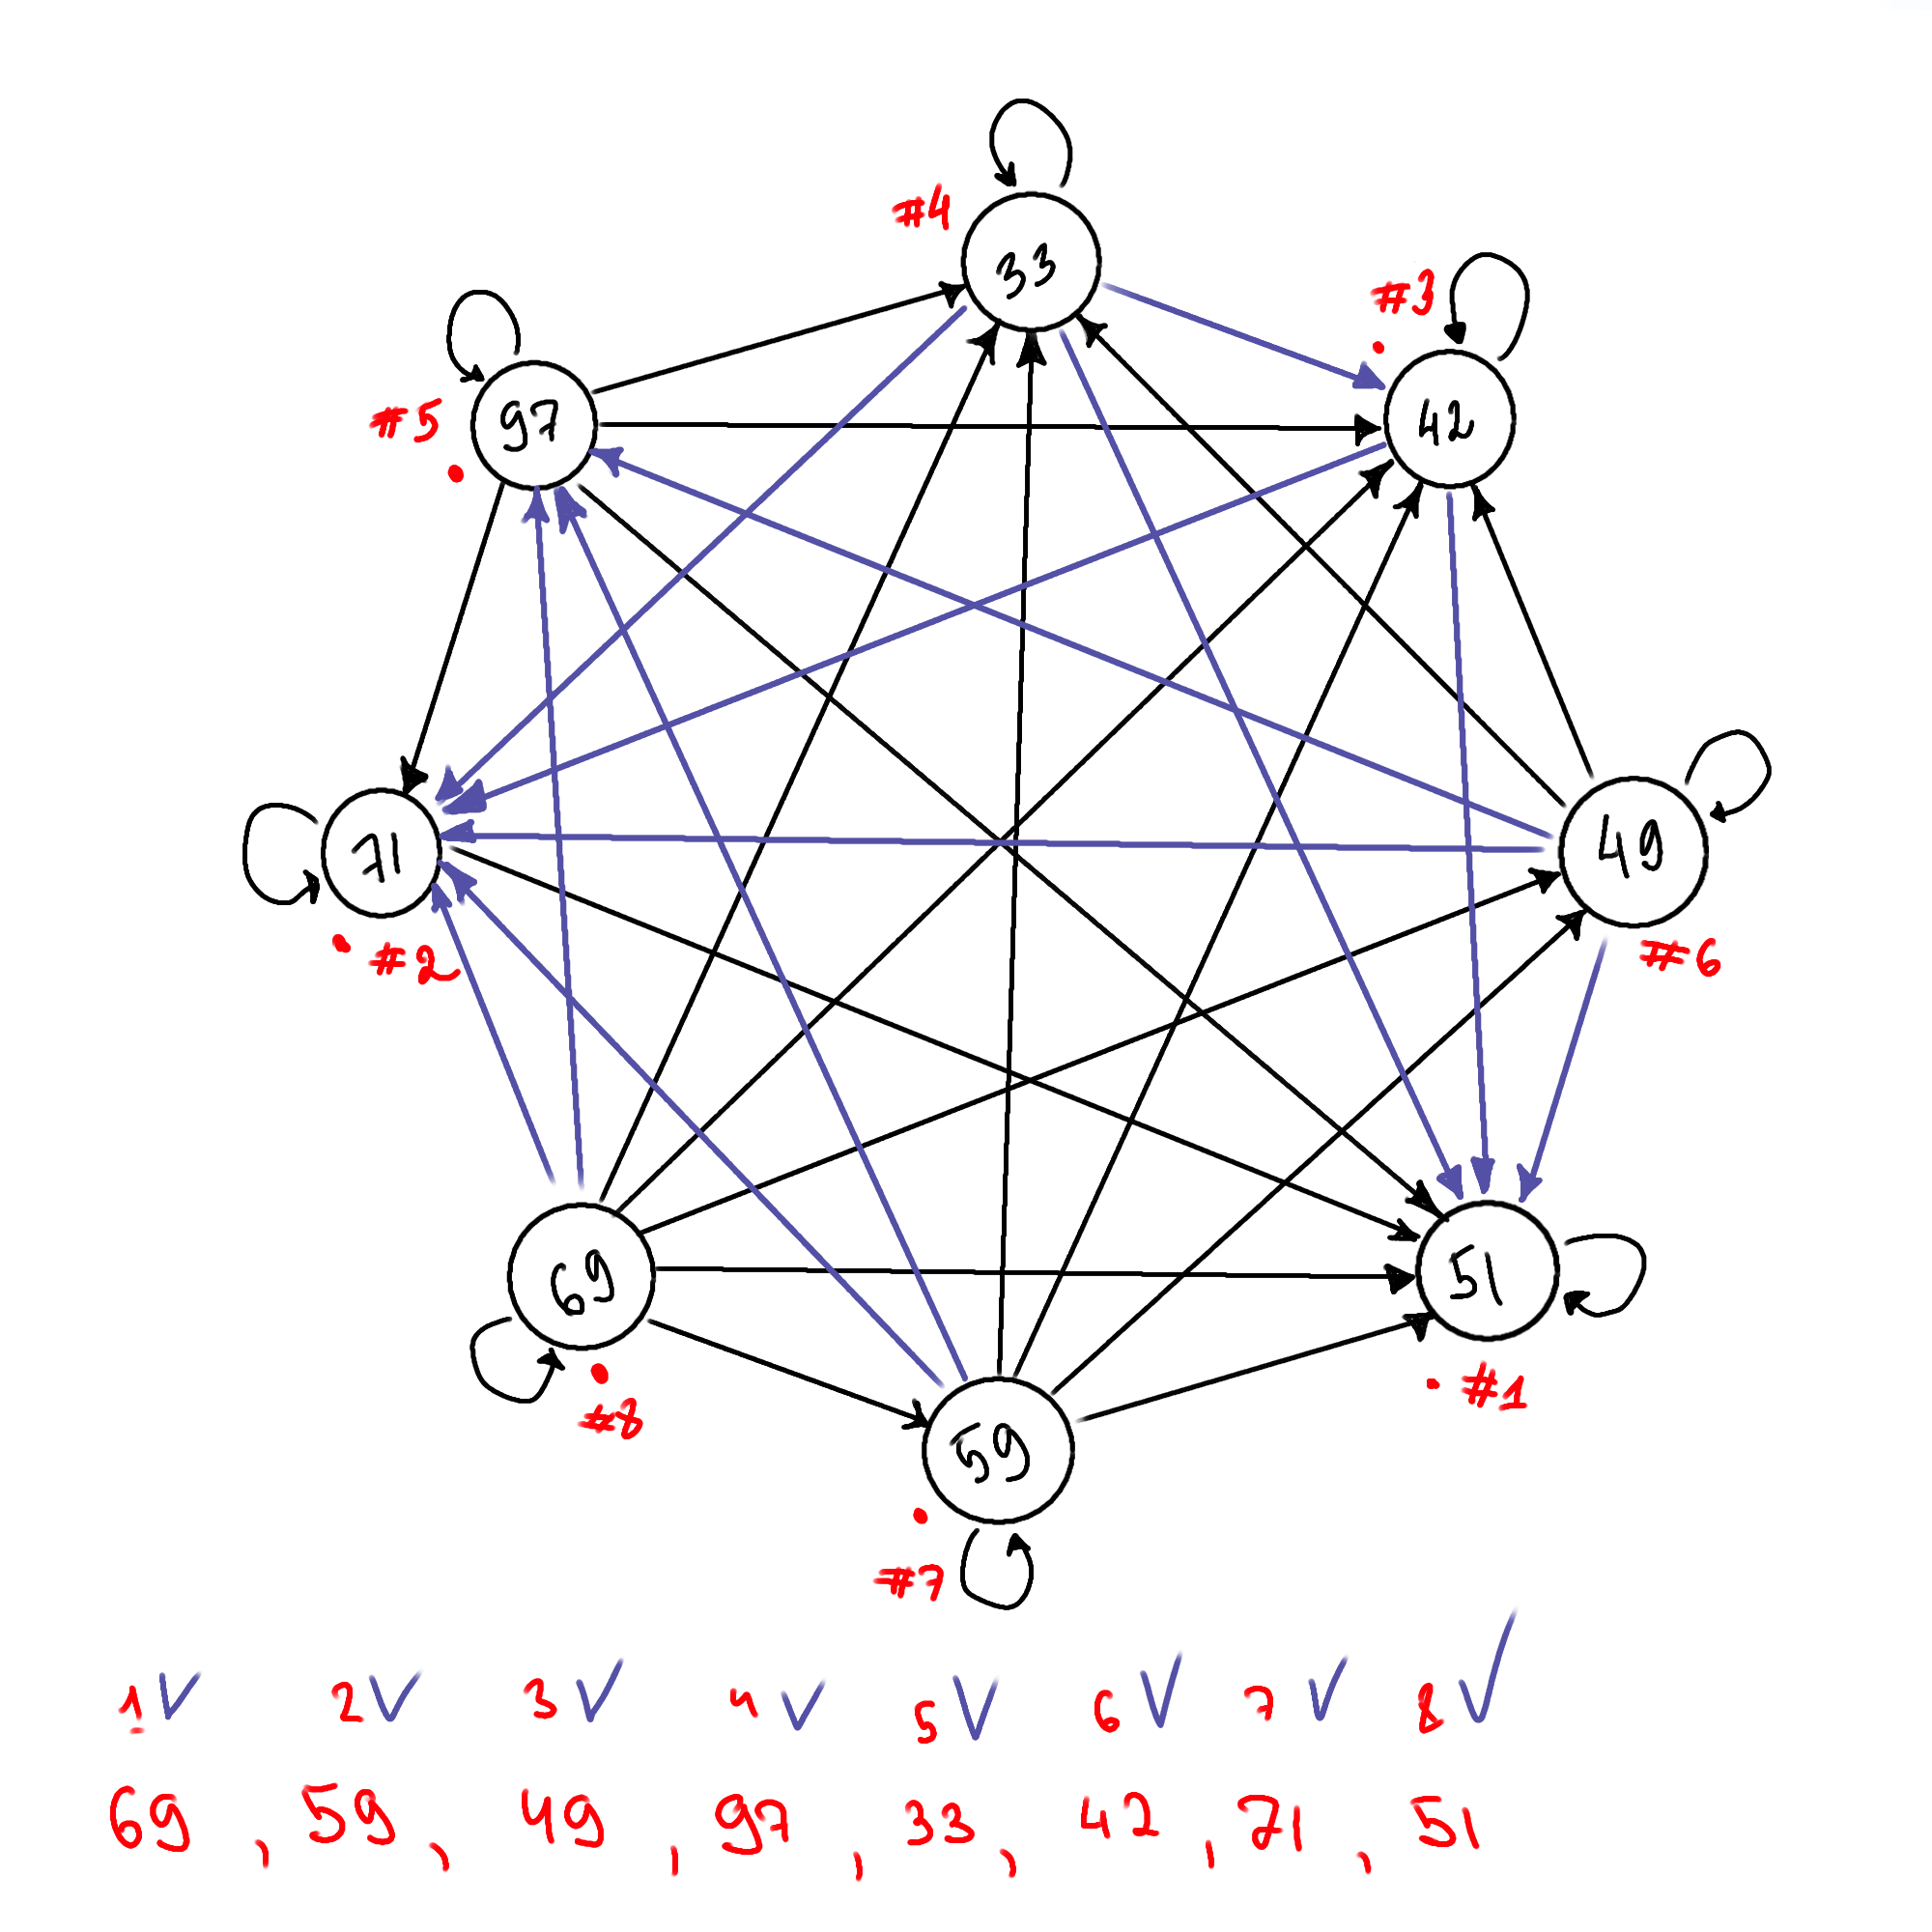
\includegraphics{сортировка.png}\newline
    3)\newline
    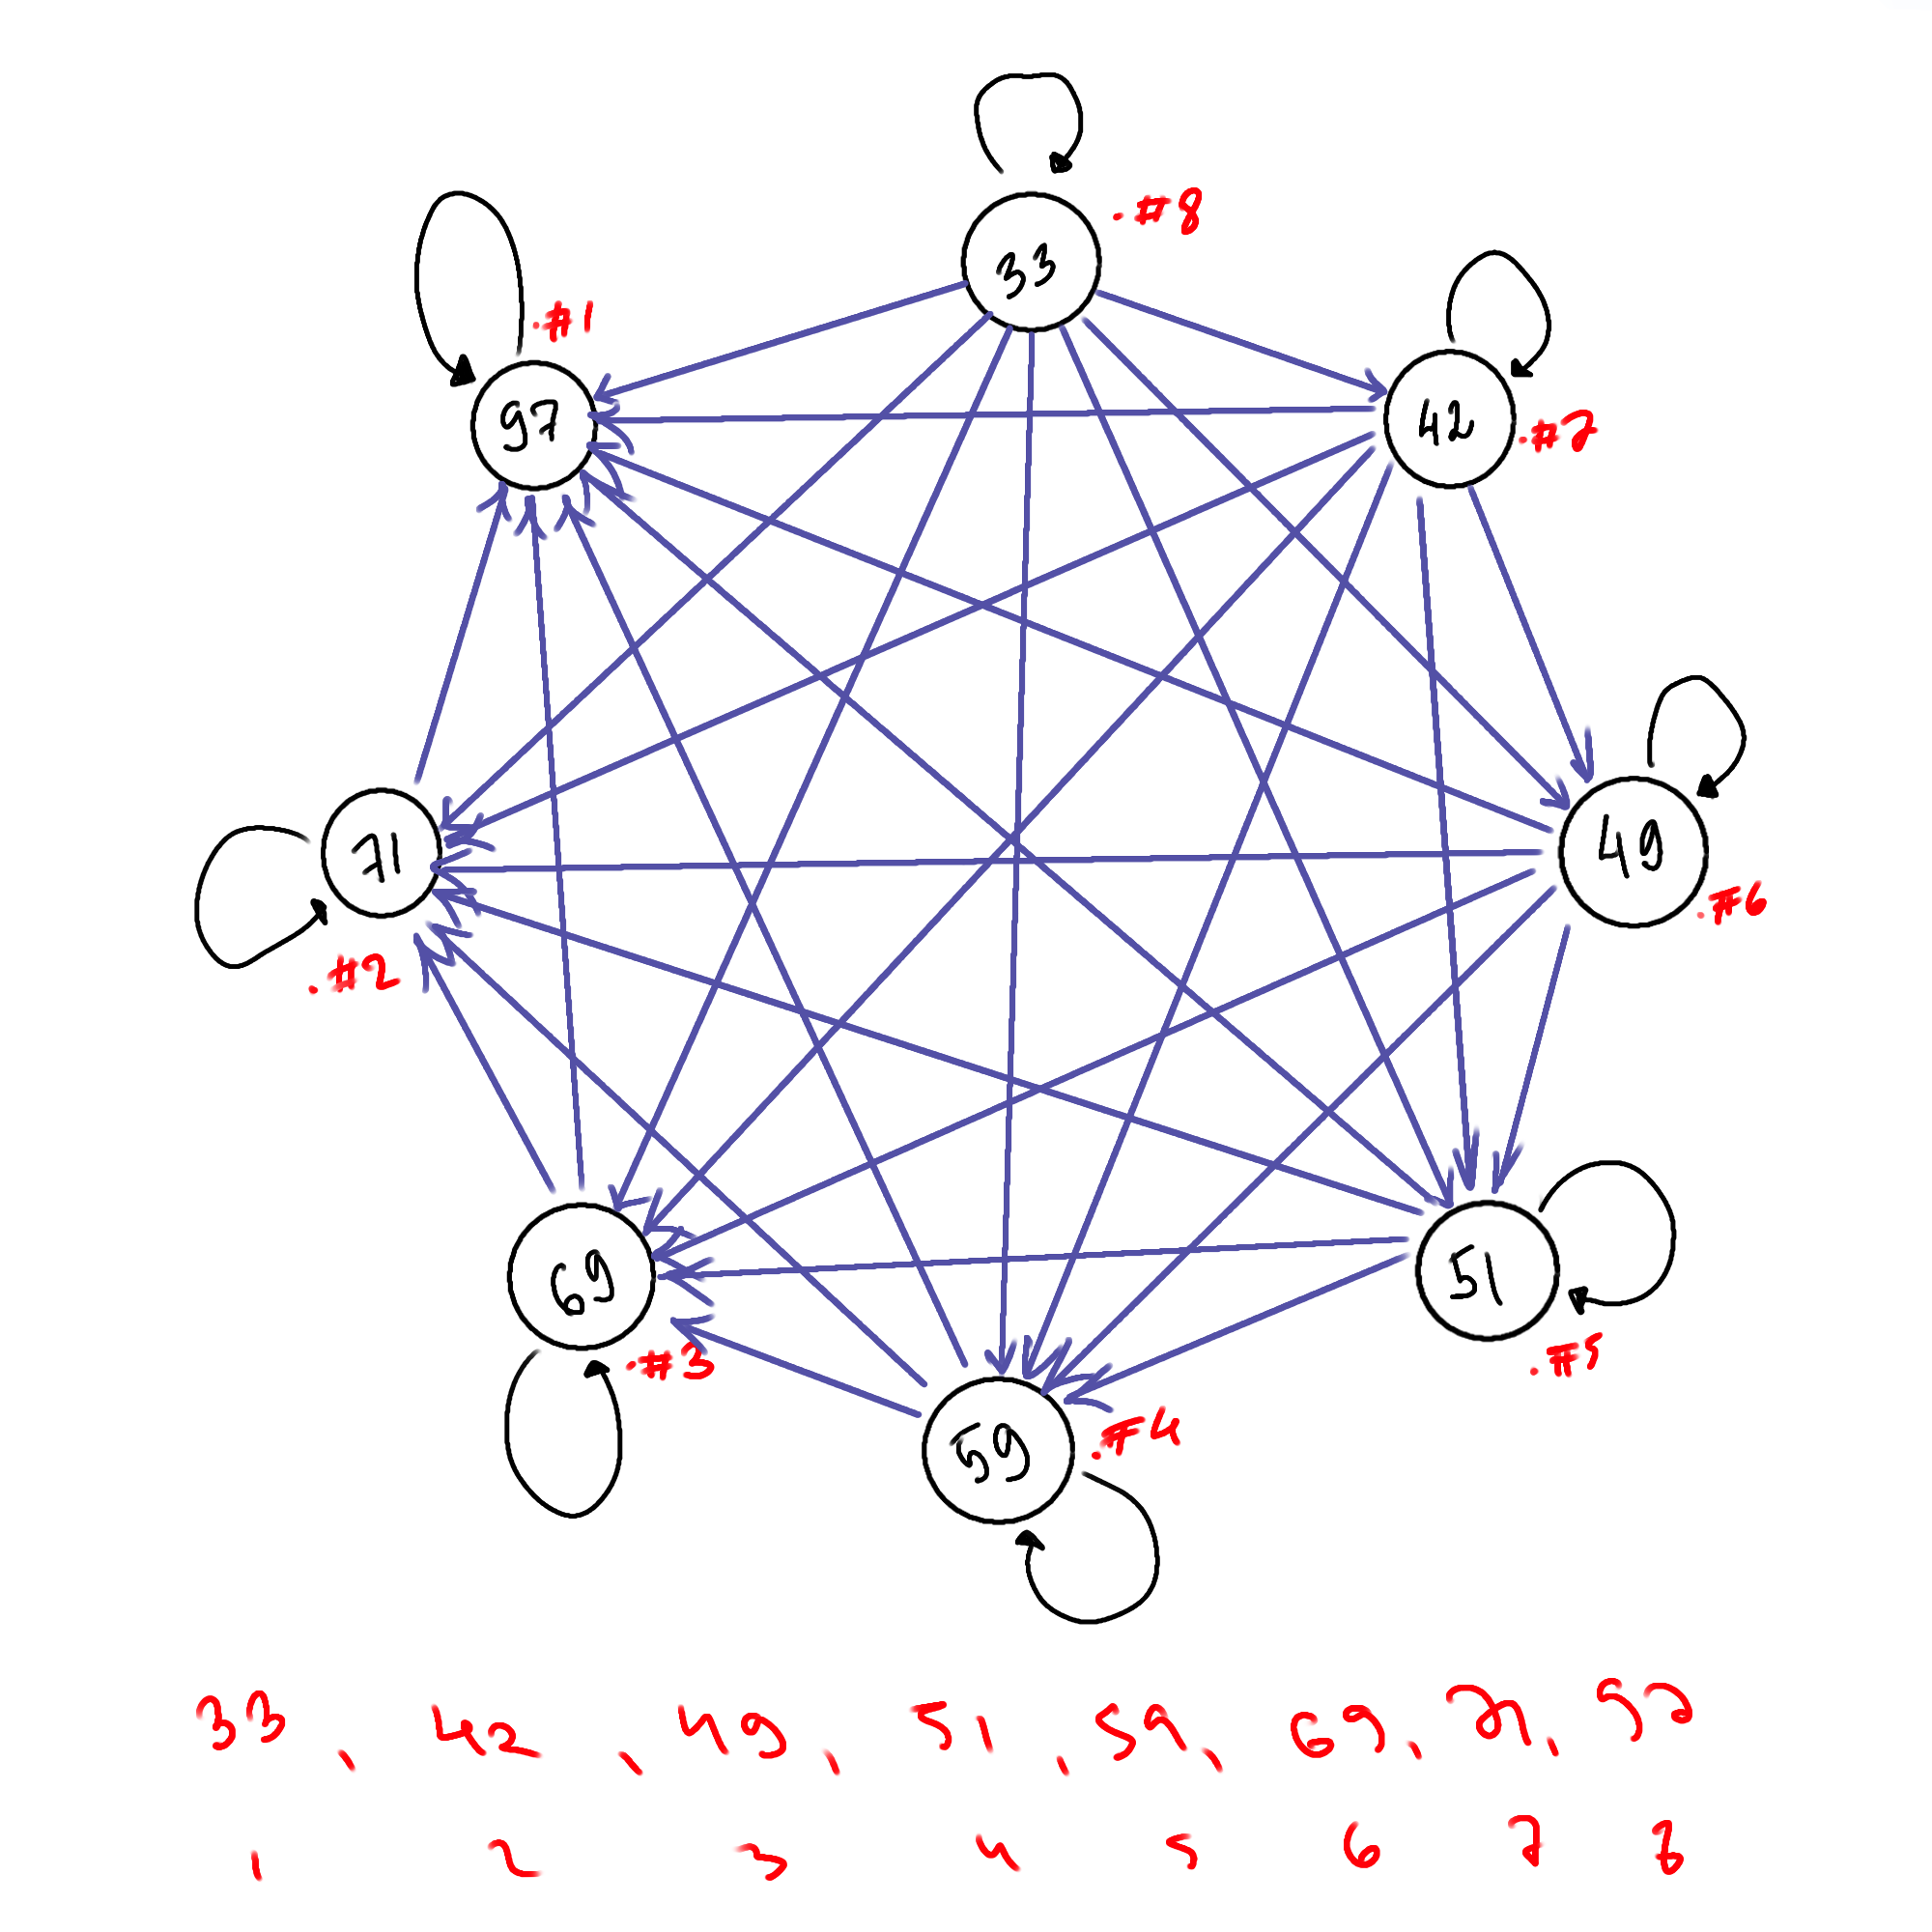
\includegraphics{сортировка2.png}\newline
    4) Б. о. не является отношением частичного порядка.\newline
    5) Б. о. не является отношением частичного порядка.\newline
\end{proof}
%%%%%%%%%%%%%% ЗАДАНИЕ №6 %%%%%%%%%%%%%%
%% Условие задания №6
\begin{problem}
	Для нетранзитивных отношений построить транзитивное замыкание, используя алгоритм Уоршелла.
\end{problem}

%% Решение задания №6
\begin{proof}
   1)\newline 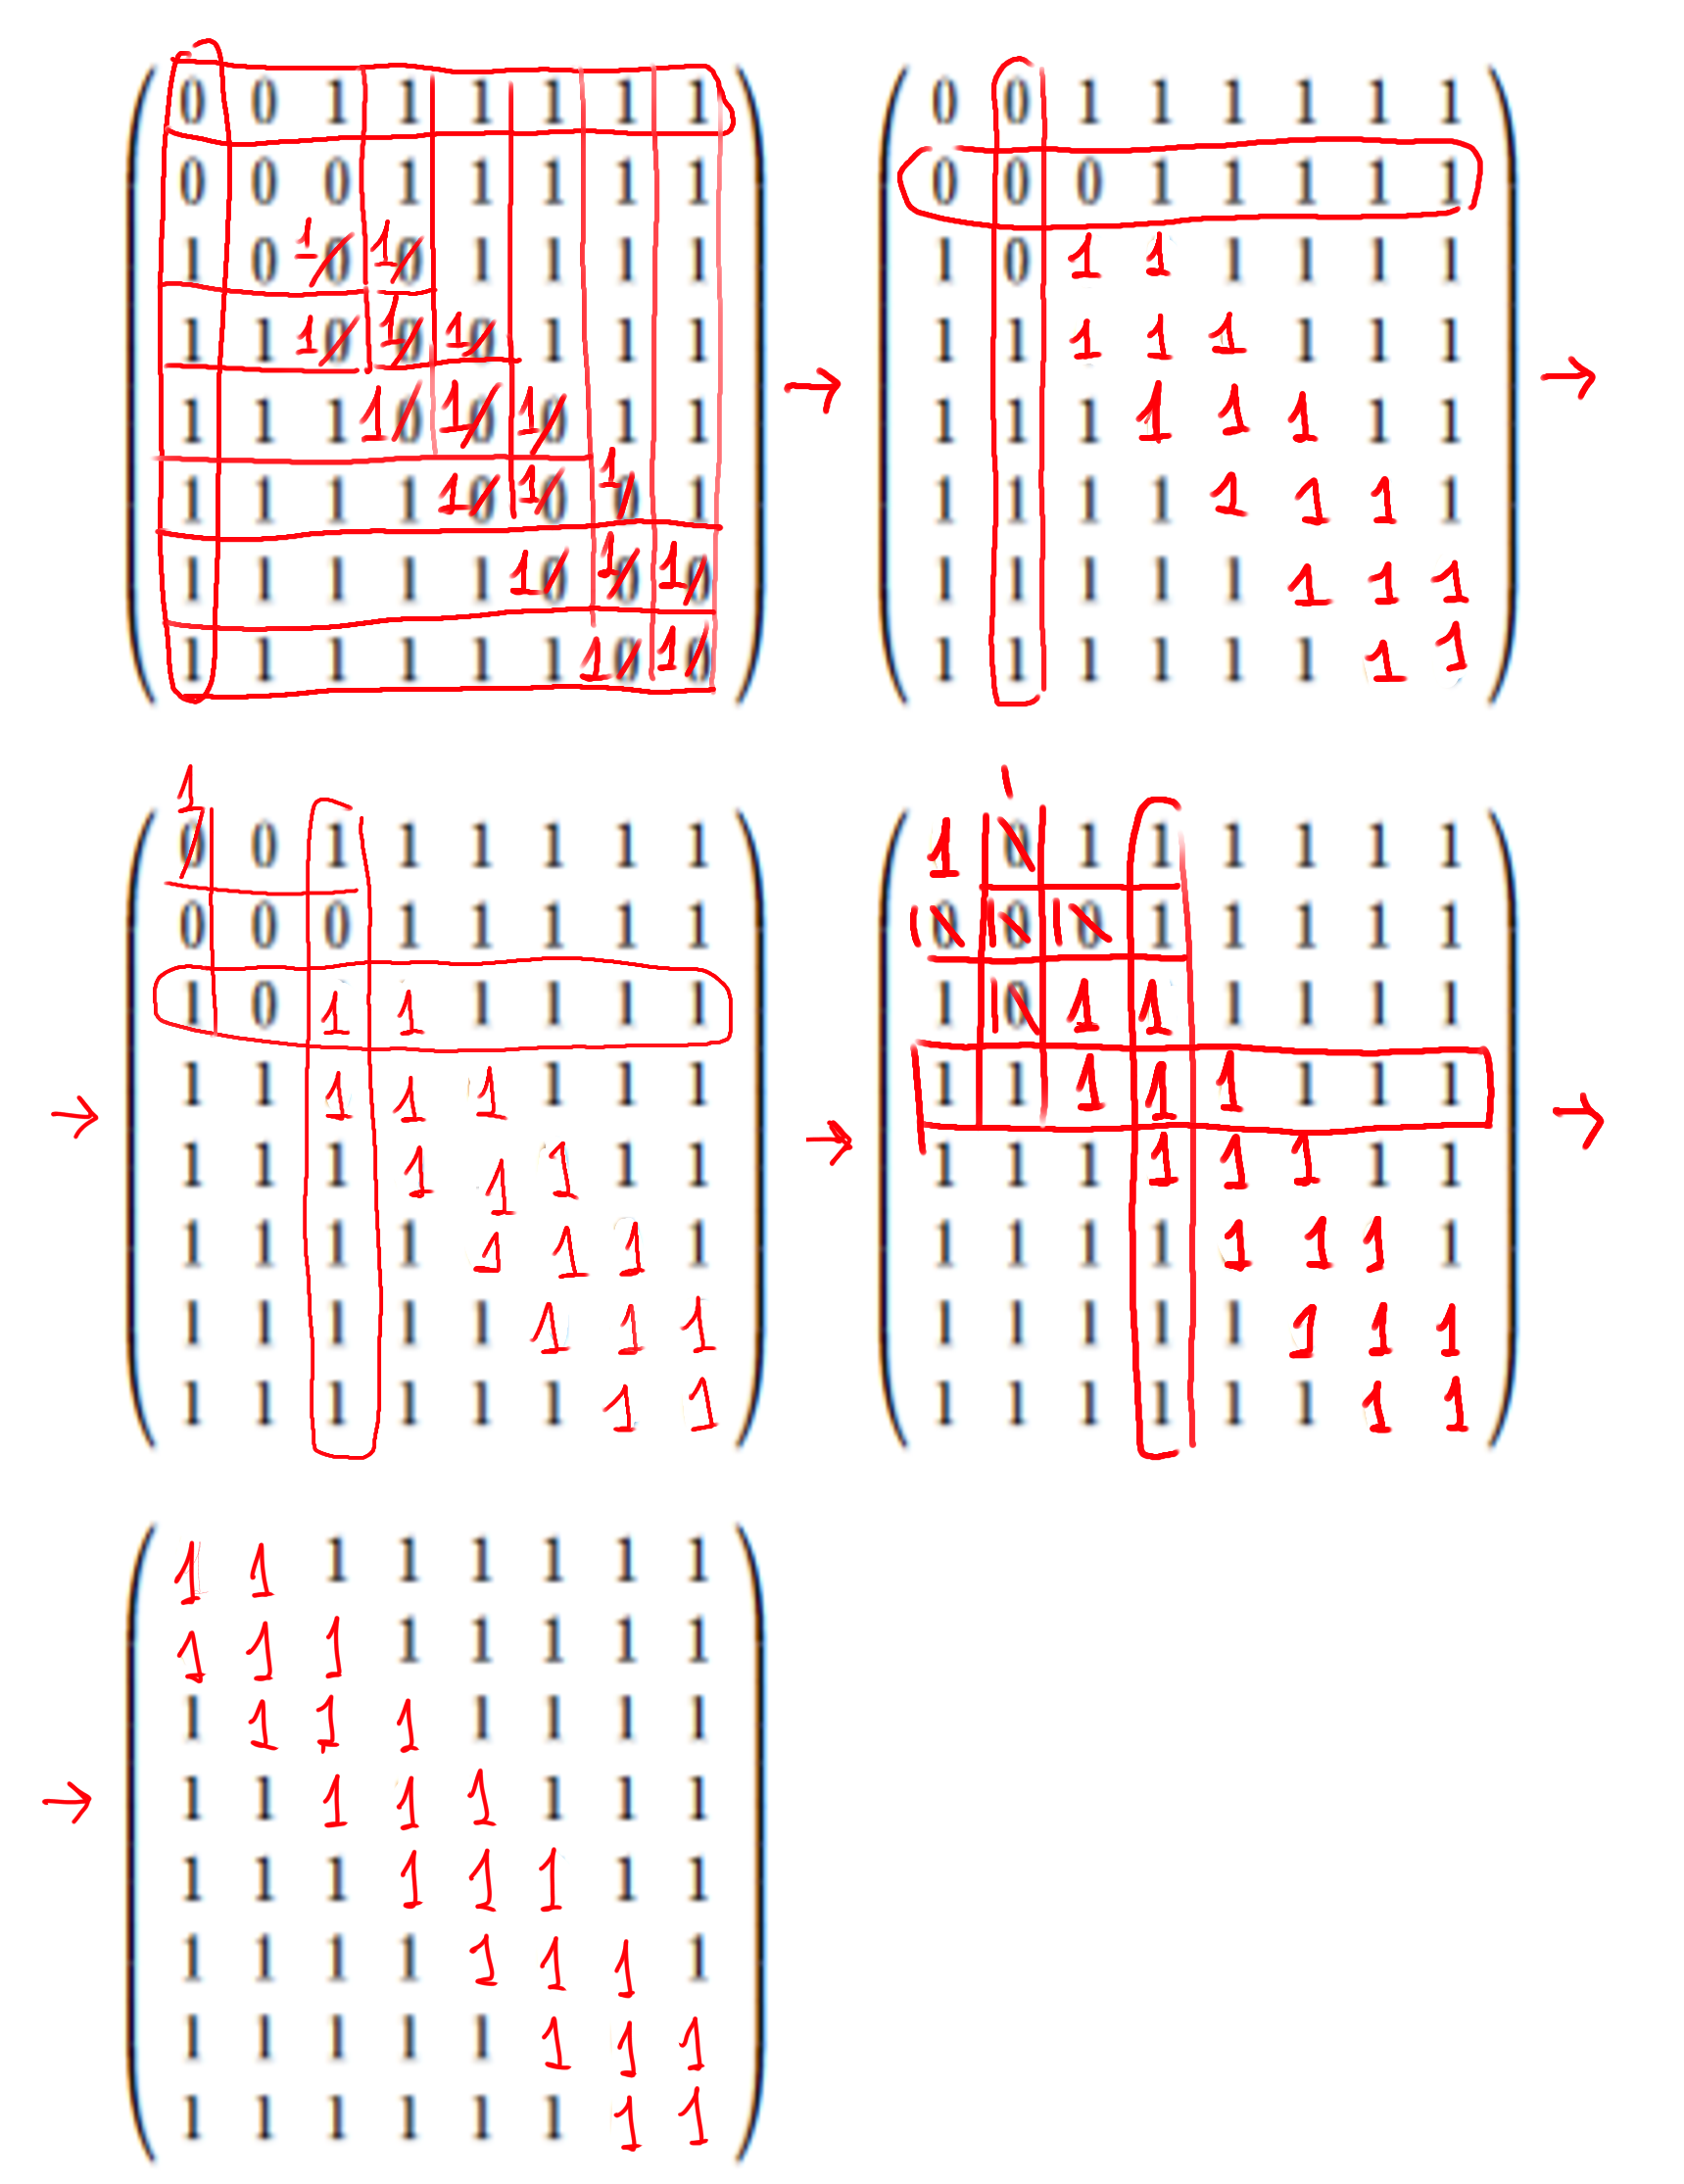
\includegraphics{замыкание.png}\newline
   2)Б.о. транзитивно.\newline
   3)Б.о. транзитивно.\newline
   4)Б.о. транзитивно.\newline
   5)Б.о. транзитивно.\newline
\end{proof}
